%% LyX 2.3.4.2 created this file.  For more info, see http://www.lyx.org/.
%% Do not edit unless you really know what you are doing.
\documentclass[english]{article}
\usepackage[T1]{fontenc}
\usepackage[utf8]{inputenc}
\usepackage{amsmath}
\usepackage{amssymb}
\usepackage{graphicx}

\makeatletter

%%%%%%%%%%%%%%%%%%%%%%%%%%%%%% LyX specific LaTeX commands.
%% Because html converters don't know tabularnewline
\providecommand{\tabularnewline}{\\}

\makeatother

\usepackage{babel}
\begin{document}
\title{How Opening Schools Influence COVID Infections -- Empirical Evidence
from Czech Republic}
\author{Martin \v Sm\'\i d, Jakub Drbohlav, Milan Zaj\'\i\v{c}ek\thanks{Institute of Information Theory and Automation of the CAS, BISOP}}
\maketitle

\section*{Main findings}
\begin{itemize}
\item Opening of schools in the Czech Republic strongly increases the infection
numbers of students
\item The effect of ordering masks in classrooms is significant in primary
schools and in secondary schools
\item Data do not support the hypothesis that the increase of reported cases
after opening schools is due to more intense testing in schools 
\item Except for kindergartens, data do not support the hypothesis that,
when being out of schools, children are infected elsewhere
\item Simple indicator of safe opening schools can be constructed. 
\item We show that hypothetical opening of schools in the middle of the
pandemics would not overturn the subsequent decreasing trend, yet
it would increase the infections significantly.
\end{itemize}

\section*{Introduction}

Closing schools during the present pandemics is the one of the most
controversial issues. According to epidemiological mainstream, schools
are strong drivers of respiratory diseases {[}cit{]}; therefore, closing
schools was one of the first governmental reactions to the outburst
of the present pandemic. However, the price we pay for closing schools
is high. Online education is not an equivalent substitute for the
in-person one; moreover, the isolation of students leaves deficit
in their necessary social contacts {[}cit{]}. Thus, for the society,
decision whether and when to close school means a painful trade-off,
making any decision political rather then scientific; science, however,
has irreplaceable role in giving the best possible (quantitative)
basis for these decisions. 

Unfortunately, it is difficult to evaluate the effect of closing schools
during the present pandemic. The virus was completely unexplored as
it came and its knowledge increased only gradually, so we only gradually
get to know, whether and how differently the virus affects children
in comparison with the rest of the population. To estimate the effect
from running epidemic data is also problematic, mainly because the
counter-epidemic measures are usually being introduced (and released)
together, so it is difficult to distinguish their effects, and even
in cases when the measures are applied in different times, still they
can be assessed only in the context of the other measures applied.
{[}Kulweit 2020{]}, for instance, regards school closure as a very
effective means of curbing the present pandemics; however, it is necessary
to take into account that school closures were usually the first measures
applied, so their measured effect may be overestimated.

In our analysis, we exploit a ``gap'' in this puzzle: the fact that
certain age cohorts of children nearly uniquely correspond to the
degrees of schools and, except for kindergartens, the majority of
children do attend their classes. Thus, it could be expected that
closing (opening) of particular degrees will result in significant
changes in infections in the corresponding cohorts. The other measures,
on the other hand, are usually much less age specific (wearing masks,
bans of gatherings) or are affecting different age cohorts (home office)
so they can be expected not to obscure the effects of school closures.
Later we show that actual data prove us right in both these assumptions
-  the effects of closures are strongly statistically significant
and the data do not exhibit co-linearity.

In the Czech Republic, all kindergartens, primary and secondary schools
had been closed on March 12, 2020, shortly after the first cases of
COVID infection appeared. While the kindergartens had been reopened
without much restriction in the beginning of May, the primary and
the secondary schools were opened during May only in a very limited
regime until the summer vacation. After the vacation, all the schools
had been opened for two weeks nearly without any restriction. Next,
after the overall incidences started to rise, wearing masks in classrooms
had been imposed. In the end of October, after serious increases of
new cases, all the schools had been closed until April 2021, except
for kindergartens, which remained open until March 2021, the first
two grades of the elementary schools, which were opened from the half
of November until February, and the final grades of the secondary
schools, which were opened one month before Christmas. On April 12th,
2021, kindergartens opened for the final year and the other schools
gradually started to be opened under rotation schemes. See the following
Table for the schedule.

\begin{tabular}{l|c|c|c|c}
Date	&	Kindergartens		&	First degree	&	Second degree	&	Secondary \\
\hline
Mar-13	&	\multicolumn{4}{c}{closed}\\
May-04	&	opened		&	closed	&	closed		&	closed \\
May-11	& & & last year max. 15 & last year  \\
May-25    &  & max. 15 voluntary & & last year max. 15 \\
% Jun-01	& &  & \\
Jun-26	&	\multicolumn{4}{c}{end of the school year} \\
Sep-01	&	\multicolumn{4}{c}{start of the school year, opened} \\
Sep-17	&	  & \multicolumn{3}{c}{masks ordered in classrooms} \\
Oct-05	&  & & & some closed \\
Oct-14	&  & \multicolumn{3}{c}{closed} \\
Nov-16	&  & open $1^{st}$ $2^{nd}$ &  &  \\
Nov-23	&  &  & & last year \\
Dec-21	&  &  & & closed \\
Mar-01	&    \multicolumn{3}{c}{closed}|\\
\end{tabular}

Unclarities:
\begin{itemize}
\item Kinergartens closed on 30 October?
\item What was open on 30 November
\item Rotations in Autumn
\end{itemize}
To evaluate the effects of the closures, we used a simple epidemiological-like
model, in which the infections in the children cohorts depend on the
overall state of epidemic plus the effect of schools, the former summand
being linearly dependent on the product of the current magnitude of
the epidemic and the current overall contact restriction, the latter
being linearly dependent on the the product the current school restrictions
and the number of infected in the cohort in question. We find the
school closures as a whole as a significant inhibitor of the epidemic,
with masks being provably efficient in the primary and secondary schools. 

Next we construct an indicator sub-unit value of which guarantees
keeping the infections in the cohort in question bounded or decreasing,
if the bound is exceeded; this indicator can serve for decisions on
school restriction degree during the epidemic.

Within the Discussion, we also discuss possible alternative explanation
of the infection increases by more extensive testing in schools, and
the hypothesis, that during school closures, children are increasingly
infected elsewhere. We find, that, except for the latter hypothesis
and kindergartens, data do not support these explanations. 

\section*{Methods}

In the Czech Republic, each September first, children who completed
their sixth year are obliged to enter the first grade of an elementary
school. When the parents wish, a child who is six as late as by the
end of the year can enter the first class, too, some children, on
the other hand, start their school later for various, mostly developmental,
reasons. If we neglect these exceptions, we can conclude that the
first year pupils are six or seven; consequently the first degree
(first five grades) pupils belong to the age cohort $6-11$. The second
degree (the sixth to the ninth year) students to the cohort $11-15$.
Finally, the students of secondary schools, which typically take four
year in the Czech Republic, belong to the cohort $15-19$. The lowest
age for admission to a kindergarten is three, so the the vast majority
of children attending kindergartens falls into the cohort $3-6$.
For simplicity we assume that the frontier one-year cohorts split
by half between the competing school categories, so the infections
happening in the cohort split by two between each category. 

Thus the number of cases by pre-school children over week $t$ in
the $i$-th district will be $X_{i,t}^{1}=Z_{i,t}^{3}+Z_{i,t}^{4}+Z_{i,t}^{5}+\frac{1}{2}Z_{i,t}^{6}$,
the number by the first degree $X_{i,t}^{2}=\frac{1}{2}Z_{i,t}^{6}+Z_{i,t}^{7}+\dots+\frac{1}{2}Z_{i,t}^{11}$,
by the second degree $X_{i,t}^{3}=\frac{1}{2}Z_{i,t}^{11}+Z_{i,t}^{12}+\dots+\frac{1}{2}Z_{i,t}^{15}$
and that by the secondary schools $X_{i,t}^{4}=\frac{1}{2}Z_{i,t}^{15}+Z_{i,t}^{16}+\dots+\frac{1}{2}Z_{i,t}^{19},$where
$Z_{i,t}^{j}$ is the number of cases by the $j$-year old individuals
in the $i$-th district. 

In line with the mainstream epidemiological modeling, we assume that
the number of overall infections $X_{i,t}$ in district $i$ is proportional
to the previous overall number of infected and the overall contact
reduction, where we take the last week incidence as a proxy for the
former:
\[
X_{t}\doteq r_{t}C_{t-1}X_{t-1};
\]
here, $C_{t-1}$ is the overall risk contact reduction within the
overall population and $r_{t}$ is the current growth rate given that
no contact reduction takes place (including the effects of virus mutations,
possible seasonal influences, natural immunization and vaccination). 

For the school children we assume that their infection consists of
a fraction of the overall infections and additional infections coming
from schools. In particular, for the $i$-th school category, 

\begin{equation}
X_{t}^{i}\doteq\alpha^{i}r_{t}C_{t}X_{t-1}+\gamma^{i}r_{t}S_{t-1}^{i}X_{t-1}^{i},\qquad S_{t-1}^{i}=D_{t-1}^{i}(1-\mu^{i}M_{t-1}^{i}),\label{eq:x}
\end{equation}
where $\alpha^{i}$ and $\gamma^{i}$ are constants, $D_{\tau}^{i}$
is the contact restriction at the school, $M_{\tau}^{i}$ is the indicator
of wearing masks in classrooms and $\mu^{i}$ is the (unknown) efficiency
of masks.

Further, assuming that, only a ratio $c$ of cases is reported, we
may divide (\ref{eq:x}) by $c$ to get 
\begin{equation}
Y_{t}\doteq r_{t}C_{t-1}Y_{t-1},\qquad Y_{t}^{i}\doteq\alpha^{i}r_{t}C_{t-1}Y_{t-1}+\gamma^{i}r_{t}S_{t-1}^{i}Y_{t-1}^{i},\qquad1\leq i\leq4,\label{eq:y}
\end{equation}
where $Y_{t}\doteq cX_{t}$ is the overall reported number of infections
and $Y_{t}^{i}\doteq cX_{t}^{i}$ is the reported infections number
in the $i$-th cohort. By dividing by the size of the cohort $i$,
we get
\begin{equation}
P_{t}^{i}\doteq\beta^{i}r_{t}C_{t-1}P_{t-1}+\gamma^{i}r_{t}S_{t-1}^{i}P_{t-1}^{i},\qquad P_{t}^{i}=\frac{Y_{t}^{i}}{s^{i}},\qquad P_{t}=\frac{Y_{t}}{s},\qquad\beta^{i}=\frac{s}{s^{i}},\label{eq:prp}
\end{equation}
where $s_{i}$ is the size of the $i$-th cohort and $s$ is the whole
population size. 

Equations (\ref{eq:y}) and (\ref{eq:prp}) may serve for understanding
of infection spread in schools and consequently for policy recommendations.
Assume that our goal is to keep new cases in the cohort less than
some $y_{0}$ (for instance, corresponding to $50$ cases per 100
thousand) and, if the number is higher, to decrease it by a ratio
$\rho_{0}$. From (\ref{eq:y}) we get that, for it to happen at $t$,
it has to be 
\[
\alpha^{i}r_{t}C_{t-1}Y_{t-1}+\gamma^{i}r_{t}S_{t-1}^{i}Y_{t-1}^{i}\leq\max(\rho_{0}Y_{t-1}^{i},y_{0})
\]
which happens if 
\[
\rho_{t}:=\rho_{t}^{\alpha}+\rho_{t}^{\gamma}<\rho_{0},\qquad\rho_{t}^{\alpha}=\alpha^{i}r_{t}C_{t-1}\frac{Y_{t-1}}{\max(Y_{t-1}^{i},y_{0})},\qquad\rho_{t}^{\gamma}=\gamma^{i}r_{t}S_{t-1}^{i}\min\left(1,\frac{Y_{t-1}^{i}}{y_{0}}\right)
\]
The equivalent formulation (\ref{eq:prp}), on the other hand, allows
comparisons between cohorts, as it speaks in the language of infection
probabilities: here the first/second summand evaluates the probability
of infection outside/inside the school. 

For the purpose of estimation, we may impose for $S_{t-1}^{i}$ in
(\ref{eq:prp}) to get a linear model 
\begin{multline}
P_{t}^{i}\doteq\beta^{i}Q_{t}+\gamma^{i}U_{t}+\delta^{i}V_{t}+\epsilon_{t},\\
Q_{t}=R_{t}P_{t},\qquad U_{t}=r_{t}D_{t-1}^{i}P_{t-1}^{i},\qquad V_{t}=r_{t}D_{t-1}M_{t-1}P_{t-1},\qquad\delta^{i}=-\mu\gamma^{i}.\label{eq:awls}
\end{multline}
Here, $\epsilon_{t}$ is centered error term for which we assume $\mathrm{var}(\epsilon_{t})\sim Q_{t}^{2}$--
see Appendix for further details and more rigorous treatment. 

\section*{Data}

Our data came from public sources. The series values $Y^{1},\dots,Y^{4},Y^{2*}$
and $Y$ are taken from the public dataset by the Czech Ministry of
Health, namely the anonymized person-level list of reported infections
(cit osoby.htm) including, among other things, the date of reporting
the infection and the age. 

The growth rate $r_{t}$ is computed by exponential smoothing of series
$\frac{Y_{t}/Y_{t-1}}{C_{t-1}}$ with parameter $\alpha=0.1,$ as
shown in the following chart. 

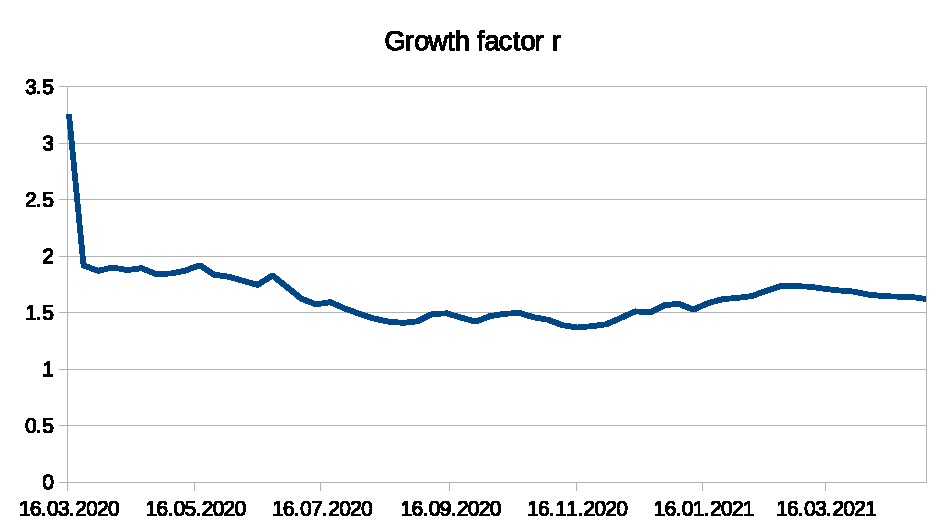
\includegraphics[scale=0.4]{r}

The values of $S$ and $M$ are estimated from publicly available
sources, mostly from resolutions of the Czech government concerning
school attendance, which have been put into effect through decrees
of the Ministry of Education (see the electronic supplement TBD for
details). Only weeks starting from April 6th, 2020 are taken into
account, as we regard the previous epidemic data as noisy, unreliable
and suffering from small sample properties. The last values correspond
to the week staring on April 5th, 2021. The values of $S$ were set
to $1$ if the school was open without any restrictions other than
mask, and to $0$ if they were closed. In the other weeks, we estimated
values of $S$ only when we could determine $S$ objectively. Thus,
we excluded observations corresponding to holidays, weeks with no
more than two possible school days, and the weeks with non-standard
regime, such as rotations or limited numbers of students in a room.
We also excluded the weeks where only first two classes had been open,
which we study separately. 

The corresponding values of $S$ and $M$ are listed in the Table
in Appendix together with the notes on how we determined fractional
values $S$ and reasons of observation exclusions. The following table
summarizes our data-set. 

\begin{tabular}{c|cccc|c}
& Kindergartens & First & Second & Secondary & First two \\
& & degree & degree & grades &  \\
\hline
Observaions &	$42$&		$23$&		$34$&		$35$&		$26$\\	 Opened &	$32$&		$7$&		$7$&		$9$&		$12$\\	 \dots with masks &		$0$&		$5$&		$5$&		$7$&		$12$\\ \dots without masks &		$32$&		$2$&		$2$&		$2$&		$0$\\  \end{tabular}

\section*{Results }

For all the cohorts with observations both with and without masks,
which are both the primary ones and the secondary one, we estimated
$\beta$,$\gamma$ and $\delta$ in (\ref{eq:awls}). In all three
cases, the coefficients came out ``reasonably'': $\beta$ came out
undoubtedly significant (overall epidemics influences the infections),
$\gamma>0$ (schools add the infections) and $0\leq-\delta\leq\gamma$
(masks reduce infection in schools). For the kindergartens, where
masks were never worn in classes, and for the first two classes, where
masks were always worn, we subsequently estimated (\ref{eq:awls})
with $\delta^{1}=0$. In both the cases, the coefficient $\gamma$
(the influence of opening) came out undoubtedly significant. 

The results of estimation may be found in the following Table. 

\begin{tabular}{c|cccc|c}
& Kindergartens & First degree & Second degree & Secondary & 1. and 2. \\ \hline
$\beta$	& $0.369^{***}(0.0578)$	& $0.55^{***}(0.0405)$	& $0.83^{***}(0.0397)$	& $0.57^{***}(0.048)$	& $0.503^{***}(0.0419)$		\\ $\gamma$	& $0.41^{***}(0.055)$	& $0.61^{**}(0.262)$	& $0.62^{***}(0.208)$	& $1.11^{***}(0.154)$	& $0.36^{***}(0.042)$		\\ $\delta$	&	& $-0.49^{*}(0.251)$	& $-0.6^{**}(0.222)$	& $-0.85^{***}(0.177)$	&		\\ \hline 
\end{tabular}

The results strongly indicate the influence of opening corresponding
school categories and they also indicate that wearing masks reduces
infections significantly. Unfortunately, due to small numbers of observations,
the estimates of $\gamma$ and $\delta$ are rather imprecise. The
values of the variance inflation factors below 5 in each case, however,
suggest that the models do not suffer from colinearity, so they should
be capable to distinguish sharply the effect of wearing masks.

When comparing the results of the individual cohorts, the values of
$\beta$, indicating the rate of infection outside schools, increase
with the age, surprisingly dropping at the secondary schools. The
values $\gamma$ (the influence of school opening without masks) increase
with age. The estimated effect of wearing masks (coefficients $\delta$)
increases with age. 

Further we focused focused on the prevailing modus operandi of the
individual school categories, namely not wearing masks in kindergartens
and wearing masks elsewhere. To this end, we re-estimated (\ref{eq:awls})
with $\delta=0$ using only records where either schools were closed
or the usual modus operandi (i.e. without masks in kindergartens,
with masks otherwise) took place. The results are in the following
table

\begin{tabular}{c|cccc|c}
& Kindergartens  & First degree & Second degree & Secondary & Primary \\ 
& no masks & masks & masks & masks & masks\\
\hline
$\beta$	& $0.369^{***}(0.0578)$	& $0.55^{***}(0.0429)$	& $0.829^{***}(0.0419)$	& $0.57^{***}(0.0425)$	& $0.503^{***}(0.0419)$	\\ $\gamma$	& $0.41^{***}(0.055)$	& $0.19^{}(0.133)$	& $0.12^{}(0.103)$	& $0.44^{***}(0.08)$	& $0.36^{***}(0.039)$	\\ \hline $\alpha$	& $0.012^{***}(0.0018)$	& $0.029^{***}(0.0023)$	& $0.035^{***}(0.0017)$	& $0.022^{***}(0.0016)$	& $0.011^{***}(0.0009)$	\\ \hline  \end{tabular}

The values and errors of $\beta$ are identical for the kindergartens
and the first grades (the same observations were used) and are nearly
identical in the remaining cases. The values of $\gamma$ are consistent
with the previous results, roughly corresponding to $\gamma-\delta$
of the previous model (in the previous model, $\gamma$ measures the
influence of not wearing masks, while here it concerns to usual modus
operandi). For the first and the second degrees, the values are insignificant,
which is non surprising, as, by the previous model, their ``true''
values are evidently too close to zero to be significant with the
present limited dataset. The (insignificant) result at the second
degree indicates less contribution than the first degree. In the secondary
schools, the contribution is again higher. 

To give the reader an idea about quantities in question, we further
plotted predictions of the ``as usual'' model for all the cohorts,
see the following Figure

\begin{tabular}{|c|c|}
\hline 
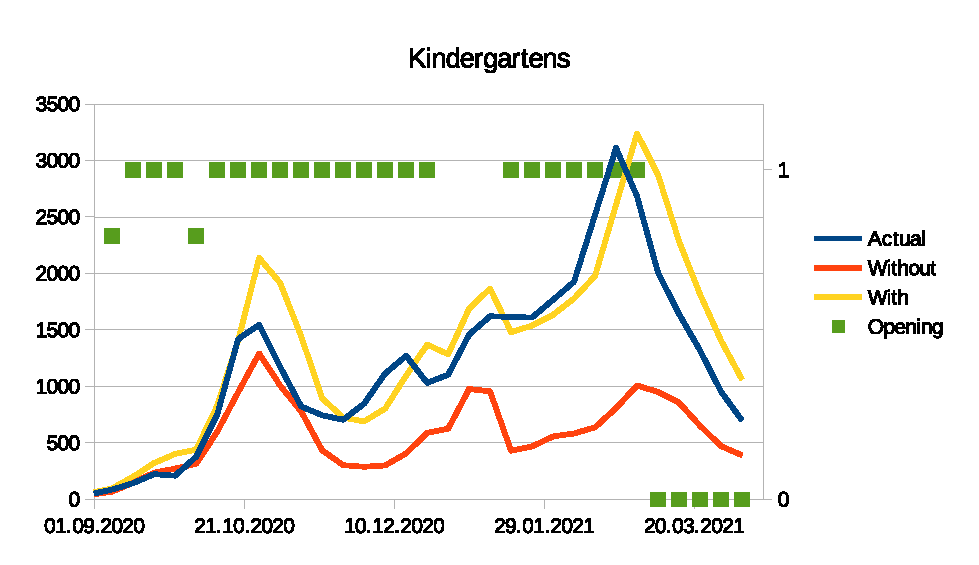
\includegraphics[scale=0.3]{k} & 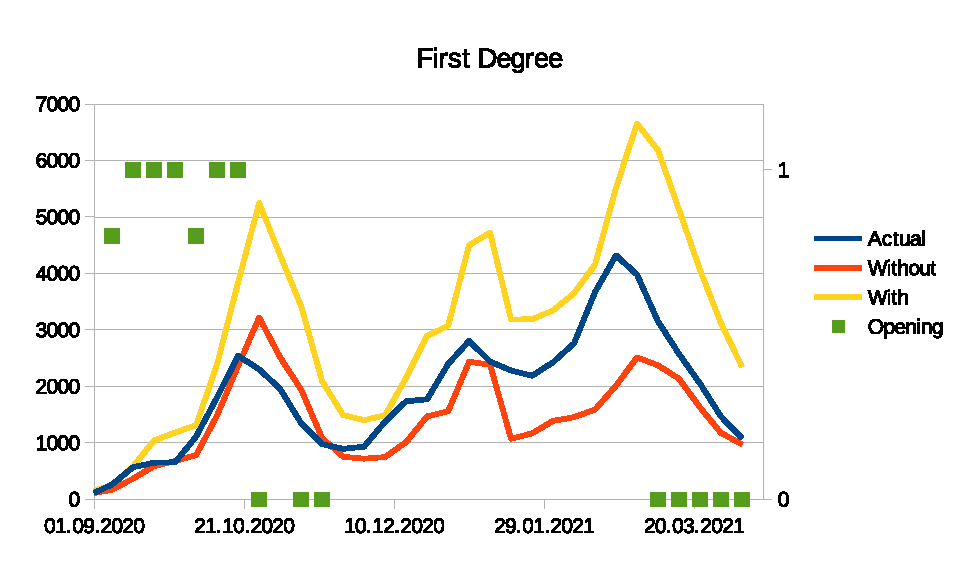
\includegraphics[scale=0.3]{fg}\tabularnewline
\hline 
\hline 
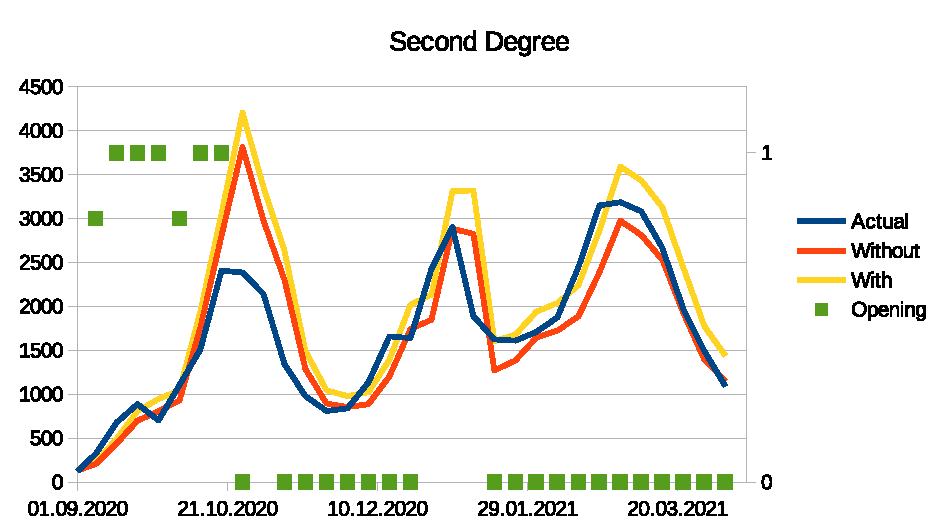
\includegraphics[scale=0.3]{sg} & 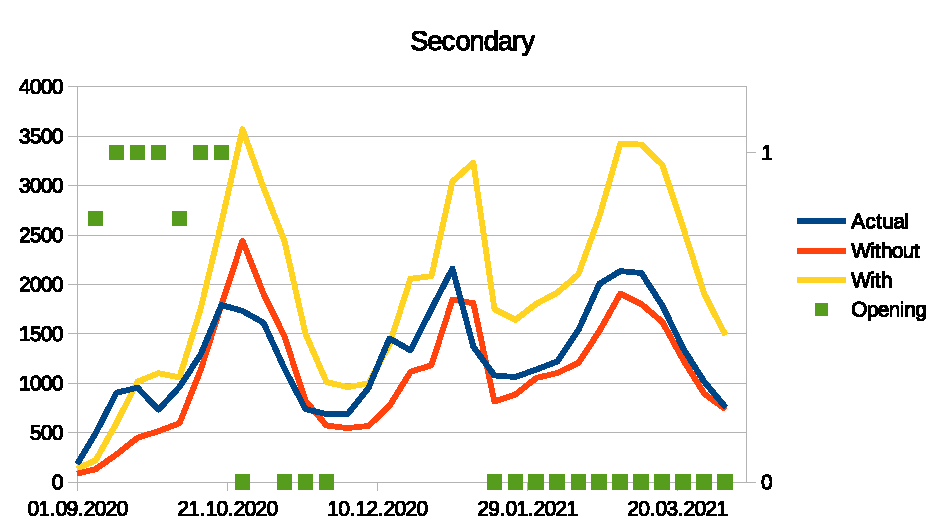
\includegraphics[scale=0.3]{sec}\tabularnewline
\hline 
\end{tabular}

The graphs show one-week predictions of $Y_{t}^{i}$ with-- and without
schools (fully) open, i.e. with $S_{t-1}=1$, $S_{t-1}=0$, respectively,
and with $M$ set according to the usual manner. In addition, actual
(observed) numbers and the degree of opening schools one week before
(values of $S_{t-1}^{i}$) are depicted. It can be seen that, according
to the model, full opening of schools (in a usual manner) at least
doubles the new cases in corresponding except for the second degrees;
however, it is important to keep in mind the insignificance of results
for the primary schools. 

Finally, we evaluated index $\rho_{t}$ for all the types during the
school year 2020/21. Recall that $\rho_{t}$ is an indicator of safe
opening of schools, whose value below $1$ indicate that the cases
in the corresponding cohort will not rise. Recall also that the indicator
is a sum of a part dependent on the outside epidemic (indexed by $\alpha$)
and the part dependent on the degree of opening of schools (indexed
by $\gamma)$. The following graphs show the values of the index through
time (with the the true degree of opening)

\begin{tabular}{|c|c|}
\hline 
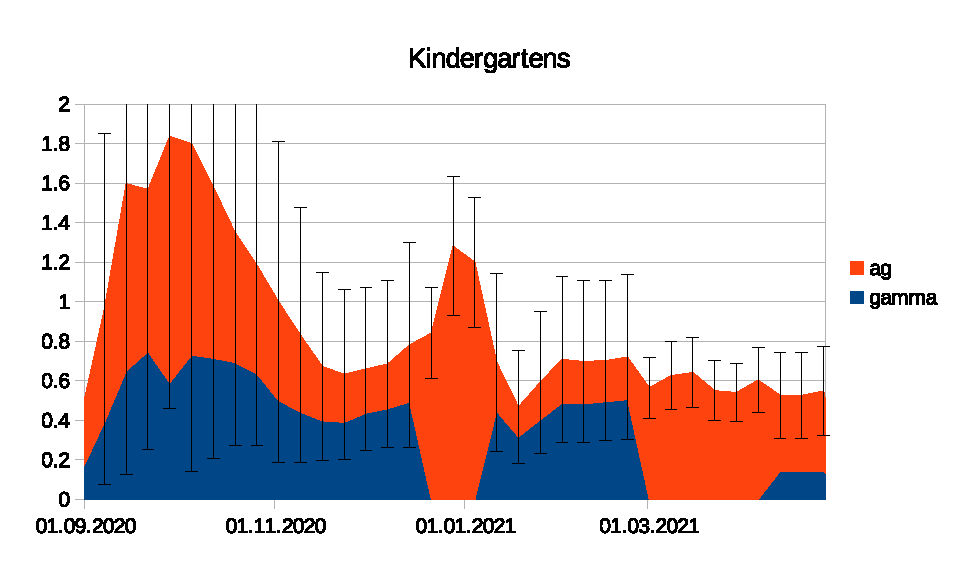
\includegraphics[scale=0.3]{rhokreal} & 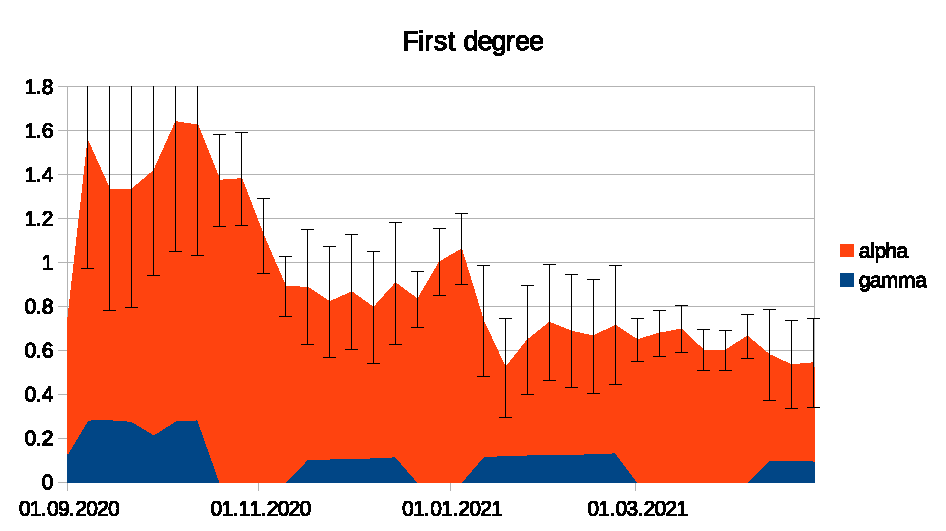
\includegraphics[scale=0.3]{rhofdreal}\tabularnewline
\hline 
\hline 
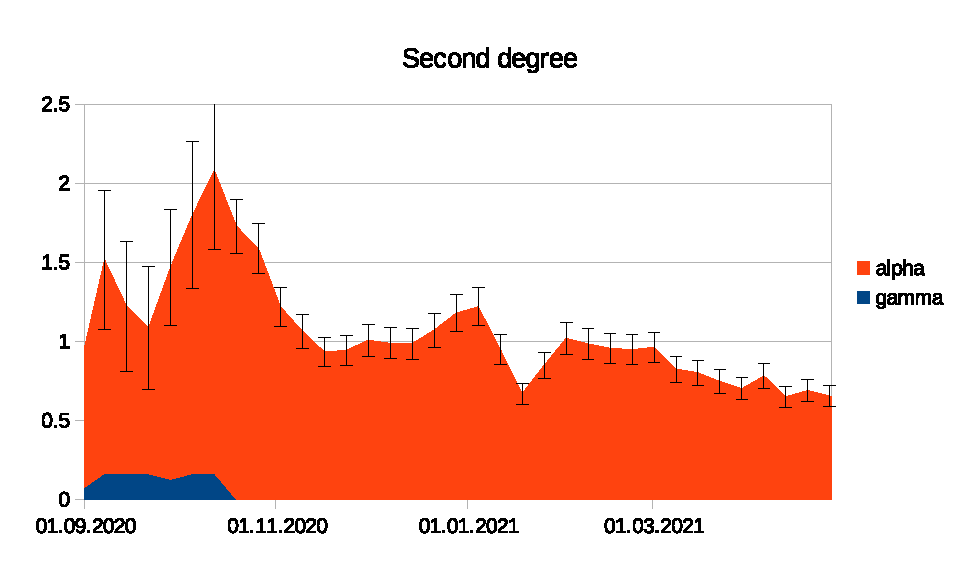
\includegraphics[scale=0.3]{rhosdreal} & 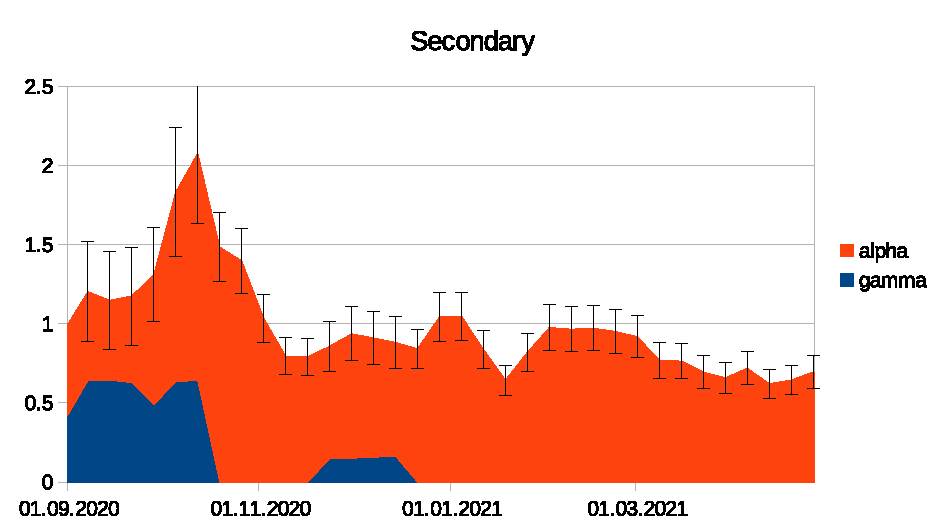
\includegraphics[scale=0.3]{rhosecreal}\tabularnewline
\hline 
\end{tabular}

Here we see that, while the closure of all types of schools may have
helped in Autumn, their closure, or not opening at least in some restricted
mode, in March seems strict. However, it should be stressed that the
indicators $\rho_{t}$ speaks only about the growth at a given time;
if the schools were open, however, the numbers of infected students
would rise, possibly amplifying the effect. To examine this, we modeled
the hypothetical situation in which all the schools were all open
(in a usual manner, i.e. with masks wherever except for kindergartens),
on March 1, which was the time when all the schools had been closed
in reality. In our forecast, we assumed the numbers of cases outside
the examined cohorts to be as in reality while the numbers in the
cohorts were computed according to the ``as usual'' model (i.e.
we neglect a possible increase outside schools due to additional infections
there). The results can be seen in the following charts.

\begin{tabular}{|c|c|}
\hline 
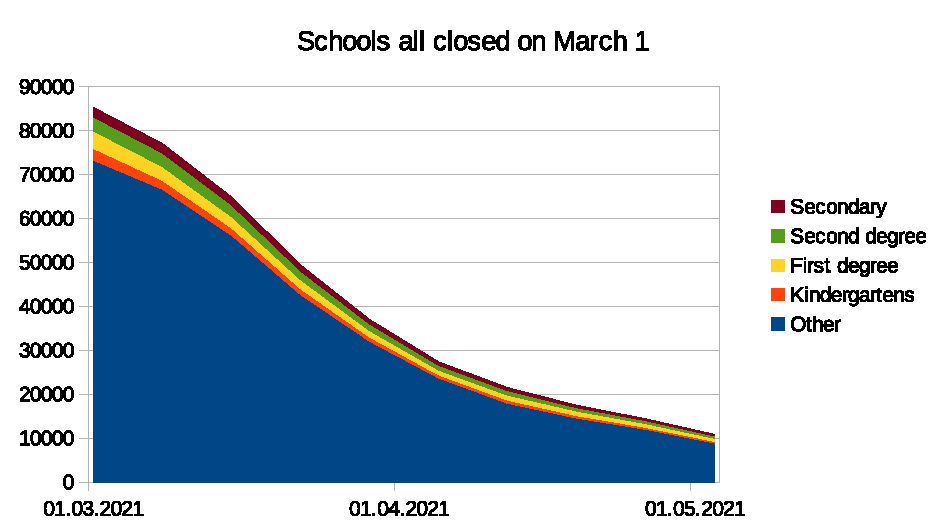
\includegraphics[scale=0.3]{marchclosed} & 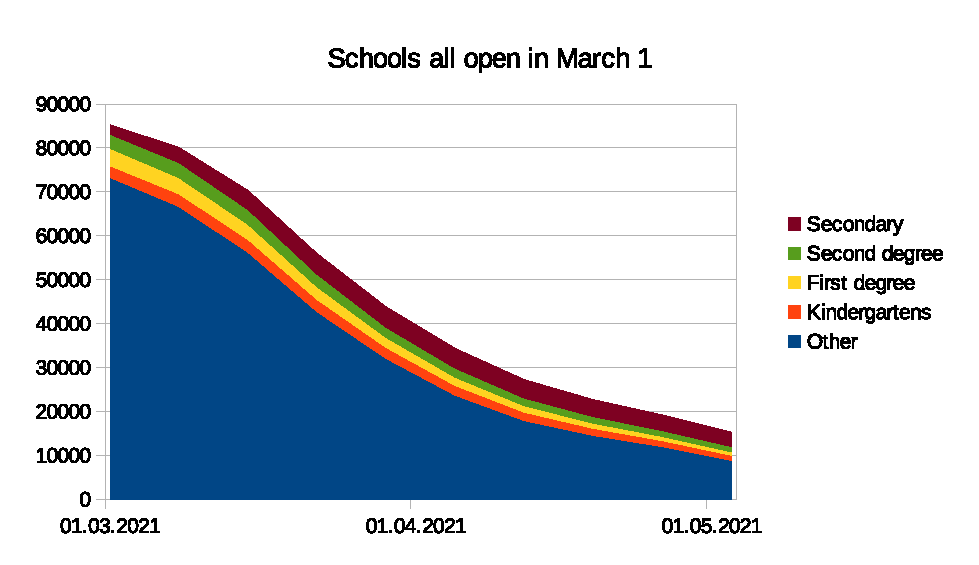
\includegraphics[scale=0.3]{marchopened}\tabularnewline
\hline 
\end{tabular}

We see in the chart, that the contribution of such opening is quite
significant and, yet it does not seem to overturn the decreasing trend
of the epidemic, it probably would, if other areas acted according
the same logic and opened too. The result however shows that, if opening
schools were politically prioritized, it would not make much harm.

\section*{Discussion}

In our honest opinion, our results convincingly prove the strong influence
of in-class education over various types of schools on the epidemic
spread, as well as its reduction by wearing masks in rooms. However,
our study has limitations. First of all it is the shortage of data.
Most of the weeks we examine the schools have been closed, and when
they were opened, mostly with masks, which clearly complicates quantification
of their influences. Therefore, the quantitative results should be
taken with slight caution.

Further, there is a determinant of children infections not taken into
account in our analysis: encounters with teachers, which can be significant
(TBD cite Neruda et al). This influence could be taken into account
by adding another coefficient into (\ref{eq:awls}); however, due
to the data shortage, there would be little chance for significant
results.

Further we discuss two arguments, often in discussions on schools:
that children, not going to schools, are infected anyway in other
environments, and that this influence of schools is spurious due to
more extensive testing of students attending schools in person, (yet,
in the examined period, no preventive testing in schools took place).
In our model, the former hypothesis would mean that, in addition to
fraction $\alpha^{i}Q_{t}$infected outside schools, $k^{i}(1-S_{t-1}^{i})Q_{t}$
for some $k^{i}$ would be infected. The latter hypothesis, on the
other hand, could be expressed as $Y_{t}^{i}=(c+S_{t-1}^{i}d^{i})X_{t}^{i}$
for some $d^{i}$. Both the hypotheses can thus be examined by estimating
a variant of the ``as usual'' model
\[
P_{t}^{i}\doteq\beta^{i}Q_{t}+\gamma^{i}U_{t}+\phi^{i}W_{t}^{i}+\eta_{t},\qquad W_{t}^{i}=Q_{t}S_{t-1}^{i};
\]
with values of $\phi^{i}<0$ speaking for the first hypothesis (children
are infected anyway), the values $\phi>0$ for the second one (there
is higher chance to be tested at school). The results of this estimation
can be found in the following Table 

\begin{tabular}{c|cccc|c}
& Kindergartens  & First degree & Second degree & Secondary & Primary \\ 
& no masks & masks & masks & masks & masks\\
\hline
$\beta$	& $0.535^{***}(0.075)$	& $0.557^{***}(0.0385)$	& $0.846^{***}(0.0454)$	& $0.578^{***}(0.0484)$	& $0.49^{***}(0.0466)$		\\ $\gamma$	& $0.49^{***}(0.058)$	& $-0.74^{}(0.467)$	& $-0.17^{}(0.339)$	& $0.4^{*}(0.22)$	& $0.35^{***}(0.047)$		\\ $\phi$	& $-0.29^{***}(0.098)$	& $0.64^{**}(0.322)$	& $0.3^{}(0.357)$	& $0.04^{}(0.305)$	& $0.04^{}(0.093)$		\\ \hline 
\end{tabular}

We can see from the table, that, for the two oldest cohorts, $\phi$
is insignificant, while, for the kindergarten cohort, results support
the hypothesis ``infected instead''. For the first degree cohort,
data suggest the ``over-tested'' hypothesis; here, however, the
result is unintuitive ($\gamma<0)$, which is probably due co-linearity
(VIR is nearing 20), invalidating the estimate of $\phi$, too. Thus,
only ``infected instead'' alternative in kindergartens should be
taken into account. However, the results are comparable here: the
following charts show the ``safety criterion'' $\rho_{t}$, which
is now changed to 

\[
\rho_{t}:=\rho_{t}^{\alpha\psi}+\rho_{t}^{\gamma}<\rho_{0},\qquad\rho_{t}^{\alpha\psi}=r_{t}(\alpha^{i}C_{t-1}+\psi^{i}S_{t-1}^{i})\frac{Y_{t-1}}{\max(Y_{t-1}^{i},y_{0})},\qquad\psi^{\acute{\imath}}=\frac{s^{i}}{s}\phi^{i}
\]
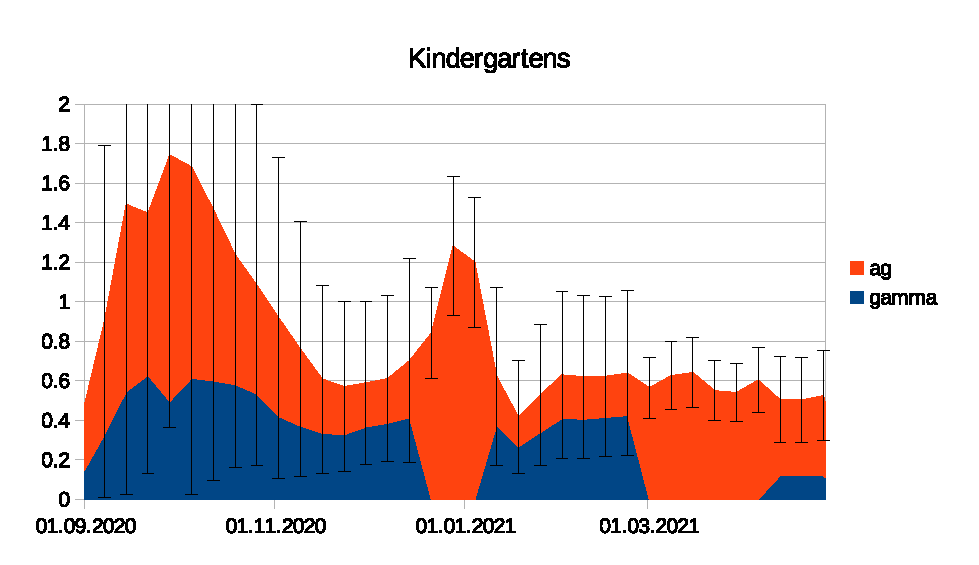
\includegraphics[scale=0.3]{rhokpsi}

\section*{Questions/Ideas}
\begin{itemize}
\item Not split primary schools (and present degrees only as secondary results)?
\end{itemize}

\section*{Appendix}

\begin{center}
\begin{table}
																	\begin{tabular}{c|cccccccc|cc}																																											 Date	&	\multicolumn{2}{c}{Kindergartens}		&	\multicolumn{2}{c}{First degree}	&	\multicolumn{2}{c}{Second degree}	&	\multicolumn{2}{c}{Secondary}	&	\multicolumn{2}{c}{Primary}	\\ \hline																															 	&	$S^1$		&	$M^1$											&	$S^2$		&	$M^2$			&	$S^3$		&	$M^3$			&	$S^4$		&	$M^4$				&	$S^{2*}$	&	$M^{2*}$		\\ \hline 06-Apr-20	&	$0$		&												&	$0$		&				&	$0$		&				&	$0$		&					&	$0$	&			\\ 13-Apr-20	&	$0$		&												&	$0$		&				&	$0$		&				&	$0$		&					&	$0$	&			\\ 20-Apr-20	&	$0$		&												&	$0$		&				&	$0$		&				&	$0$		&					&	$0$	&			\\ 27-Apr-20	&	$0$		&												&	$0$		&				&	$0$		&				&	$0$		&					&	$0$	&			\\ 04-May-20	&	$1$		&	N											&	$0$		&				&	$0$		&				&	$0$		&					&	$0$	&			\\ 11-May-20	&	$1$		&	N											&	$0$		&				&	$\times^{ad}$		&				&	$0.25^{d}$		&	Y				&	$0$	&			\\ 18-May-20	&	$1$		&	N											&	$0$		&				&	$\times^{ad}$		&				&	$0.25^{d}$		&	Y				&	$0$	&			\\ 25-May-20	&	$1$		&	N											&	$\times^{a}$		&				&	$\times^{ad}$		&				&	$\times^{ad}$		&					&	$\times$	&			\\ 01-Jun-20	&	$1$		&	N											&	$\times^{a}$		&				&	$\times^{ad}$		&				&	$\times^{ad}$		&					&	$\times$	&			\\ 08-Jun-20	&	$1$		&	N											&	$\times^{a}$		&				&	$\times^{ad}$		&				&	$0$		&					&	$\times$	&			\\ 15-Jun-20	&	$1$		&	N											&	$\times^{a}$		&				&	$\times^{ad}$		&				&	$0$		&					&	$\times$	&			\\ 22-Jun-20	&	$1$		&	N											&	$\times^{a}$		&				&	$\times^{ad}$		&				&	$0$		&					&	$\times$	&			\\ 29-Jun-20	&	$\times^{e}$		&												&	$\times^{e}$		&				&	$\times^{e}$		&				&	$\times^{e}$		&					&	$\times$	&			\\ 	&	$\vdots$		&												&	$\vdots$		&				&	$\vdots$		&				&	$\vdots$		&					&	$\times$	&			\\ 																																										
																																										
																																										
																																										
																																										
																																										
24-Aug-20	&	$\times^{e}$		&												&	$\times^{e}$		&				&	$\times^{e}$		&				&	$\times^{e}$		&					&	$\times$	&			\\ 31-Aug-20	&	$0.8^{a}$		&	N											&	$0.8^{b}$		&	N			&	$0.8^{b}$		&	N			&	$0.8^{b}$		&	N				&	$0.8$	&		N	\\ 07-Sep-20	&	$1$		&	N											&	$1$		&	N			&	$1$		&	N			&	$1$		&	N				&	$1$	&		N	\\ 14-Sep-20	&	$1$		&	N											&	$1^{I}$		&	N			&	$1^{I}$		&	N			&	$1^{I}$		&	N				&	$1$	&		N	\\ 21-Sep-20	&	$1$		&	N											&	$1$		&	Y			&	$1$		&	Y			&	$1$		&	Y				&	$1$	&		Y	\\ 28-Sep-20	&	$0.8^{a}$		&	N											&	$0.8^{b}$		&	Y			&	$0.8^{b}$		&	Y			&	$0.8^{b}$		&	Y				&	$0.8$	&		Y	\\ 05-Oct-20	&	$1$		&	N											&	$1$		&	Y			&	$1$		&	Y			&	$\times^{j}$		&					&	$1$	&		Y	\\ 12-Oct-20	&	$1$		&	N											&	$\times^{h}$		&				&	$\times^{h}$		&				&	$\times^{h}$		&					&	$\times$	&			\\ 19-Oct-20	&	$1$		&	N											&	$0$		&				&	$0$		&				&	$0$		&					&	$0$	&			\\ 26-Oct-20	&	$1$		&	N											&	$\times^{g}$		&				&	$\times^{g}$		&				&	$\times^{g}$		&					&	$\times$	&			\\ 02-Nov-20	&	$1$		&	N											&	$0$		&				&	$0$		&				&	$0$		&					&	$0$	&			\\ 09-Nov-20	&	$1$		&	N											&	$0$		&				&	$0$		&				&	$0$		&					&	$0$	&			\\ 16-Nov-20	&	$1$		&	N											&	$\times^{c}$		&				&	$0$		&				&	$0$		&					&	$1$	&		Y	\\ 23-Nov-20	&	$1$		&	N											&	$\times^{c}$		&				&	$0$		&				&	$\times^{d}$		&					&	$1$	&		Y	\\ 30-Nov-20	&	$1$		&	N											&	$\times^{c}$		&				&	$0$		&				&	$\times^{d}$		&					&	$1$	&		Y	\\ 07-Dec-20	&	$1$		&	N											&	$\times^{c}$		&				&	$0$		&				&	$\times^{d}$		&					&	$1$	&		Y	\\ 14-Dec-20	&	$1$		&	N											&	$\times^{c}$		&				&	$0$		&				&	$\times^{d}$		&					&	$1$	&		Y	\\ 21-Dec-20	&	$\times^{f}$		&												&	$\times^{f}$		&				&	$\times^{f}$		&				&	$\times^{f}$		&					&	$\times$	&			\\ 28-Dec-20	&	$\times^{f}$		&												&	$\times^{f}$		&				&	$\times^{f}$		&				&	$\times^{f}$		&					&	$\times$	&			\\ 04-Jan-21	&	$\times^{f}$		&												&	$\times^{f}$		&				&	$\times^{f}$		&				&	$\times^{f}$		&					&	$\times$	&			\\ 11-Jan-21	&	$1$		&	N											&	$\times^{c}$		&				&	$0$		&				&	$0$		&					&	$1$	&		Y	\\ 18-Jan-21	&	$1$		&	N											&	$\times^{c}$		&				&	$0$		&				&	$0$		&					&	$1$	&		Y	\\ 25-Jan-21	&	$1$		&	N											&	$\times^{c}$		&				&	$0$		&				&	$0$		&					&	$1$	&		Y	\\ 01-Feb-21	&	$1$		&	N											&	$\times^{c}$		&				&	$0$		&				&	$0$		&					&	$1$	&		Y	\\ 08-Feb-21	&	$1$		&	N											&	$\times^{c}$		&				&	$0$		&				&	$0$		&					&	$1$	&		Y	\\ 15-Feb-21	&	$1$		&	N											&	$\times^{c}$		&				&	$0$		&				&	$0$		&					&	$1$	&		Y	\\ 22-Feb-21	&	$1$		&	N											&	$\times^{c}$		&				&	$0$		&				&	$0$		&					&	$1$	&		Y	\\ 01-Mar-21	&	$0$		&												&	$0$		&				&	$0$		&				&	$0$		&					&	$0$	&			\\ 08-Mar-21	&	$0$		&												&	$0$		&				&	$0$		&				&	$0$		&					&	$0$	&			\\ 15-Mar-21	&	$0$		&												&	$0$		&				&	$0$		&				&	$0$		&					&	$0$	&			\\ 22-Mar-21	&	$0$		&												&	$0$		&				&	$0$		&				&	$0$		&					&	$0$	&			\\ 29-Mar-21	&	$0$		&												&	$0$		&				&	$0$		&				&	$0$		&					&	$0$	&			\\ 05-Apr-21	&	$0$		&												&	$0$		&				&	$0$		&				&	$0$		&					&	$0$	&			\\ \end{tabular}																																											 																													 																 \caption{Notes: a -- voluntary, only 15 pupils in the classroom (approx. half), b -- only 4 days from week, c -- only 1st and 2nd calsses are open, d -- only the last year open, e -- summer vacation, f -- Christmas vacation, g -- autumn vacation,  h -- closed on Wednsday, i -- masks ordered from Thuersday, j -- closed in more affected regions }																				 \end{table}															
\end{center}																	 

\section*{The Statistical Model}

TBD

\end{document}

Our goal is to examine whether opening of schools contributes to the
epidemic and whether masks play role in schools. To this end we assume
that the expected weekly number number of newly infected children
of the $i$-th cohort outside schools is Compound Poisson with mean
\[
\beta_{t}^{i}X_{t-1},\qquad X_{t-1}=\sum_{j=1}^{5}X_{t-1}^{j},\qquad\beta_{t}=R_{t}\beta,
\]
where $\beta$ is an unknown constant and $R_{t}$ the reproduction
number.

Further, we hypothesize that the number of children of the $i$-th
cohort, infected at school, is Compound Poisson with mean 

\[
\gamma_{t}^{i}(1-M_{t-1}^{i}\mu)S_{t-1}^{i}X_{t-1}^{i}\qquad\gamma_{t}^{i}=r_{t}\gamma^{i}
\]
where $\mu^{i}$ is an unknown efficiency of masks, $\gamma^{i}$
is an unknown constant and $r_{t}=R_{t}/C_{t-2}$ is the the basic
reproduction number, 

The logic behind our model is following: without schools, the cohort
of interest is infected ``as usual'' which means that the rate of
their infection is proportional to the reproduction number and the
number of infected in the whole population (a proxy for which up to
constant is the daily number of infected). In schools, the situation
is similar with the difference that we explicitly model the contact
intensity therein (by variables $S$ and $M$ and constants $\gamma$
and $\delta$), so the reproduction number has to be stripped of the
influence of the overall contact restriction; therefore, we assume
the infection to be proportional to $r$ rather than to $R$.

Summed up, we have 

\begin{multline*}
X_{t}^{i}=\beta_{t}^{i}X_{t-1}+\gamma_{t}^{i}(1-M_{t-1}^{i}\mu^{i})S_{t-1}^{i}X_{t-1}^{i}+\epsilon_{t}^{i}\\
=\beta^{i}R_{t}X_{t-1}+\gamma^{i}r_{t}S_{t-1}^{i}X_{t-1}^{i}+\delta^{i}r_{t}M_{t-1}^{i}S_{t-1}^{i}X_{t-1}^{i}+\epsilon_{t}^{i},\qquad\delta^{i}=\gamma^{i}\mu^{i}.
\end{multline*}
where $\mathbb{E}\epsilon_{t}^{i}=0$ and $\mathrm{var}(\epsilon_{t}^{i})$
is, up to a constant, equal to the r.h.s. minus the residuum.

Finally, we assume that the observed numbers $Y_{t}^{1},\dots,Y_{t}^{5}$
of the infected are proportional to the actual ones, namely $Y_{t}^{i}=cX_{t}^{i}+e_{t}^{i}$
where $c$ is an unknown constant and $e_{t}^{t}$ are centered with
$\mathrm{var(e_{t}^{i})\sim}X_{t}^{i}$. This gives

\begin{multline*}
Y_{t}^{i}=\beta^{i}I_{t}+\gamma^{i}U_{t}^{i}+\delta^{i}V_{t}^{i}+\eta_{t}^{i},\qquad I_{t}=R_{t}Y_{t-1},\qquad U_{t}^{i}=r_{t}S_{t-1}^{i}Y_{t-1}^{i},\qquad V_{t}^{i}=r_{t}M_{t-1}^{i}S_{t-1}^{i}Y_{t-1}^{i}\\
\eta_{t}^{i}=\frac{\epsilon_{t}^{i}}{c}+r_{t}\left[\beta^{i}\sum_{j=1}^{k}e_{t}^{j}+(\gamma^{i}S_{t-1}^{i}+\delta^{i}M_{t-1}^{i}S_{t-1}^{i})e_{t}^{i}\right]
\end{multline*}
Note that $\mathbb{\ensuremath{E}}\eta_{t}^{i}=0$ and $\mathrm{var(}\eta_{i}^{i})=\sum_{j}d_{t}^{i,j}X_{t}^{j}$
for some $d_{i,t}^{t}$. As, in practice, the ratio of $X_{t}^{i}$
does not vary much in time, we approximate $\text{var}(\eta_{i}^{i})\doteq dX_{t}\doteq\frac{d}{c}I_{t}$
where $d$ is unknown parameter. 

Our hypotheses are 

\[
H_{0}^{i}:\gamma^{i}=0\text{ against }H_{1}^{i}:\gamma^{i}>0
\]
(schools do not/do have influence) and 
\[
\tilde{H}_{0}^{i}:\delta^{i}=0\text{ against }\tilde{H}_{1}^{i}:\delta^{i}<0
\]
(masks do not / do have influence).

We use WLS to estimate coefficients in (\ref{eq:wls}), i.e. OLS after
dividing the equation by $\sqrt{I_{t}}$ for each $t$, and test the
hypotheses by $t$-tests for each $i.$
\end{document}
